\documentclass[11pt,a4paper]{article}
\usepackage[margin=2.2cm]{geometry}
\usepackage{amsmath,amssymb}
\usepackage{graphicx}
\usepackage{booktabs}
\usepackage{hyperref}
\usepackage{tikz}
\usetikzlibrary{arrows.meta,positioning,shapes.geometric,calc,fit,backgrounds}
\usepackage{xcolor}
\usepackage{enumitem}
\usepackage{float}
\usepackage{caption}
\usepackage{longtable}
\usepackage{tabularx}
\usepackage{multirow}

% Colors
\definecolor{realistic}{HTML}{2E8B57}
\definecolor{simplified}{HTML}{DAA520}
\definecolor{missing}{HTML}{CD5C5C}
\definecolor{brainblue}{HTML}{4682B4}
\definecolor{modelorange}{HTML}{E8751A}
\definecolor{lightgray}{HTML}{F0F0F0}

\hypersetup{colorlinks=true, linkcolor=brainblue, citecolor=brainblue, urlcolor=brainblue}

\title{\textbf{Biological Plausibility Assessment:\\Virtual Zebrafish Brain v2}}
\author{Hae-Jeong Park\\Department of Nuclear Medicine, Yonsei University College of Medicine}
\date{March 2026}

\begin{document}
\maketitle

%% ========================================================================
\begin{abstract}
We present an honest biological plausibility assessment of the Virtual Zebrafish Brain v2,
a spiking neural network model comprising 7,369 Izhikevich neurons organized into
tectum, thalamus, pallium, basal ganglia, amygdala, and reticulospinal modules.
The model uses conductance-based synapses (AMPA, NMDA, GABA\textsubscript{A}) with
Mg$^{2+}$ block, three-factor STDP with eligibility traces, and predictive coding
feedback between pallium layers.  Connectome constraints are drawn from the MapZebrain
atlas (Kunst et al., 2019).
In standardized decision-quality benchmarks the model achieves 77/100,
demonstrating competent foraging, flee, and exploration behavior.
However, the model uses approximately 50$\times$ fewer neurons than the real
zebrafish brain ($\sim$100K), employs point neurons without dendritic computation or
gap junctions, and relies on analytic Expected Free Energy (EFE) formulas rather than
emergent spiking dynamics for goal selection.
Several brain regions---habenula, cerebellum, hypothalamus---are entirely absent.
This report maps every model component to its biological counterpart, identifies what
is genuinely realistic, what is simplified, and what is missing, providing a roadmap
for future improvements toward greater biological fidelity.
\end{abstract}

\tableofcontents
\newpage

%% ========================================================================
\section{Zebrafish Brain Anatomy vs.\ Model Architecture}
\label{sec:anatomy}

\subsection{Architecture Comparison Figure}

Figure~\ref{fig:architecture} provides a side-by-side comparison of the real larval
zebrafish brain and the v2 model architecture.  Solid colored lines indicate
implemented projections; dashed gray lines indicate known biological connections
that are missing from the model.

\begin{figure}[H]
\centering
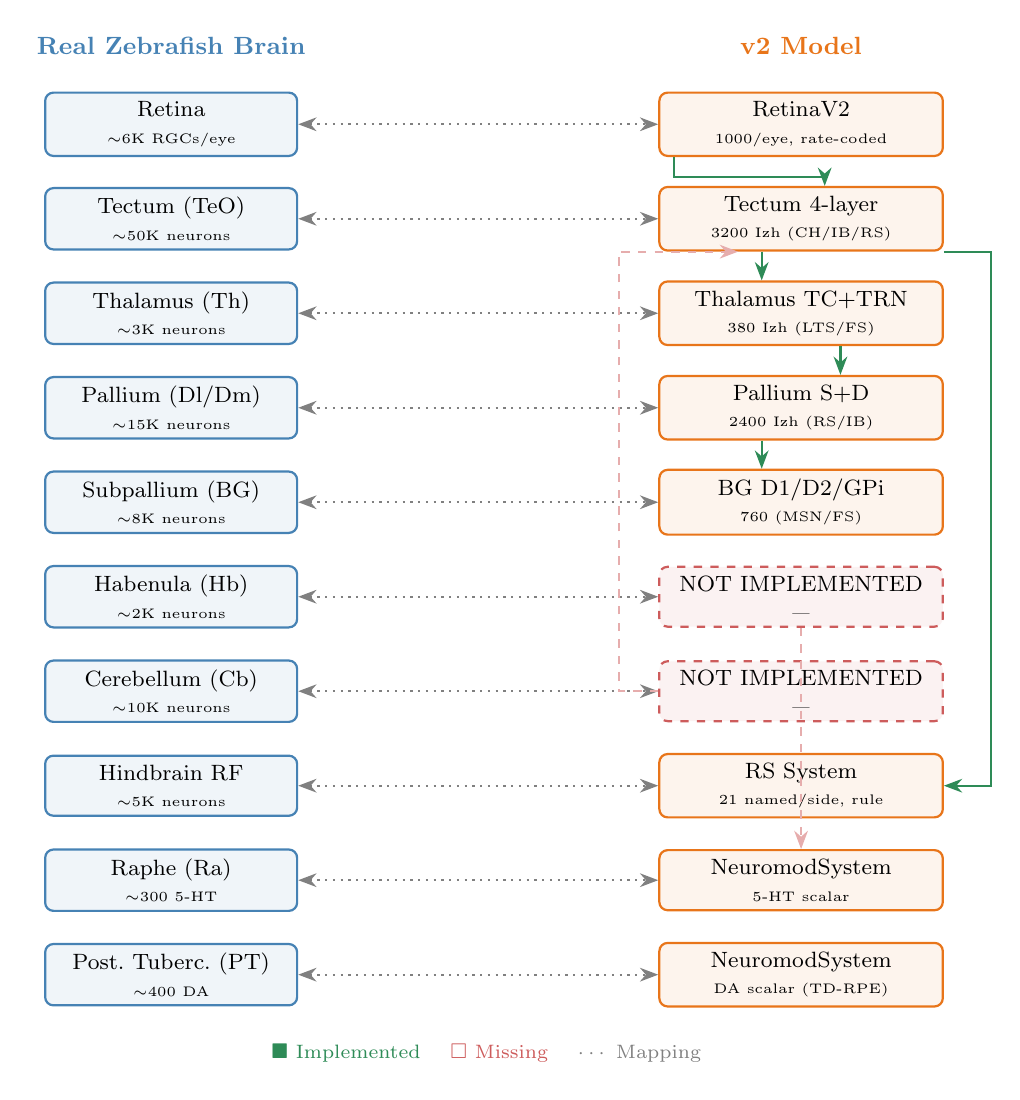
\begin{tikzpicture}[
    >=Stealth,
    brainbox/.style={draw=brainblue, fill=brainblue!8, rounded corners=3pt,
                     minimum width=3.2cm, minimum height=0.65cm, font=\footnotesize,
                     align=center, thick},
    modelbox/.style={draw=modelorange, fill=modelorange!8, rounded corners=3pt,
                     minimum width=3.6cm, minimum height=0.65cm, font=\footnotesize,
                     align=center, thick},
    missingbox/.style={draw=missing, fill=missing!8, rounded corners=3pt,
                       minimum width=3.6cm, minimum height=0.65cm, font=\footnotesize,
                       align=center, thick, dashed},
    impl/.style={->, thick, color=realistic},
    miss/.style={->, thick, color=missing!50, dashed},
    map/.style={<->, dotted, color=gray, thick},
]
% Title labels
\node[font=\bfseries\small, color=brainblue] at (-3.8, 7.0) {Real Zebrafish Brain};
\node[font=\bfseries\small, color=modelorange] at (4.2, 7.0) {v2 Model};

% ---- LEFT: Real brain regions ----
\node[brainbox] (retina) at (-3.8, 6.0) {Retina\\{\tiny $\sim$6K RGCs/eye}};
\node[brainbox] (teo)    at (-3.8, 4.8) {Tectum (TeO)\\{\tiny $\sim$50K neurons}};
\node[brainbox] (th)     at (-3.8, 3.6) {Thalamus (Th)\\{\tiny $\sim$3K neurons}};
\node[brainbox] (pal)    at (-3.8, 2.4) {Pallium (Dl/Dm)\\{\tiny $\sim$15K neurons}};
\node[brainbox] (sp)     at (-3.8, 1.2) {Subpallium (BG)\\{\tiny $\sim$8K neurons}};
\node[brainbox] (hb)     at (-3.8, 0.0) {Habenula (Hb)\\{\tiny $\sim$2K neurons}};
\node[brainbox] (cb)     at (-3.8, -1.2) {Cerebellum (Cb)\\{\tiny $\sim$10K neurons}};
\node[brainbox] (rf)     at (-3.8, -2.4) {Hindbrain RF\\{\tiny $\sim$5K neurons}};
\node[brainbox] (ra)     at (-3.8, -3.6) {Raphe (Ra)\\{\tiny $\sim$300 5-HT}};
\node[brainbox] (pt)     at (-3.8, -4.8) {Post.\ Tuberc.\ (PT)\\{\tiny $\sim$400 DA}};

% ---- RIGHT: v2 Model modules ----
\node[modelbox] (m_ret)  at (4.2, 6.0) {RetinaV2\\{\tiny 1000/eye, rate-coded}};
\node[modelbox] (m_tec)  at (4.2, 4.8) {Tectum 4-layer\\{\tiny 3200 Izh (CH/IB/RS)}};
\node[modelbox] (m_th)   at (4.2, 3.6) {Thalamus TC+TRN\\{\tiny 380 Izh (LTS/FS)}};
\node[modelbox] (m_pal)  at (4.2, 2.4) {Pallium S+D\\{\tiny 2400 Izh (RS/IB)}};
\node[modelbox] (m_bg)   at (4.2, 1.2) {BG D1/D2/GPi\\{\tiny 760 (MSN/FS)}};
\node[missingbox] (m_hb) at (4.2, 0.0) {NOT IMPLEMENTED\\{\tiny ---}};
\node[missingbox] (m_cb) at (4.2, -1.2) {NOT IMPLEMENTED\\{\tiny ---}};
\node[modelbox] (m_rs)   at (4.2, -2.4) {RS System\\{\tiny 21 named/side, rule}};
\node[modelbox] (m_5ht)  at (4.2, -3.6) {NeuromodSystem\\{\tiny 5-HT scalar}};
\node[modelbox] (m_da)   at (4.2, -4.8) {NeuromodSystem\\{\tiny DA scalar (TD-RPE)}};

% ---- Mapping arrows ----
\draw[map] (retina.east) -- (m_ret.west);
\draw[map] (teo.east)    -- (m_tec.west);
\draw[map] (th.east)     -- (m_th.west);
\draw[map] (pal.east)    -- (m_pal.west);
\draw[map] (sp.east)     -- (m_bg.west);
\draw[map] (hb.east)     -- (m_hb.west);
\draw[map] (cb.east)     -- (m_cb.west);
\draw[map] (rf.east)     -- (m_rs.west);
\draw[map] (ra.east)     -- (m_5ht.west);
\draw[map] (pt.east)     -- (m_da.west);

% ---- Implemented connections (right side) ----
\draw[impl] (m_ret.south west) ++(0.2,0) -- ++(0,-0.25) -| ([xshift=0.3cm]m_tec.north);
\draw[impl] ([xshift=-0.5cm]m_tec.south) -- ([xshift=-0.5cm]m_th.north);
\draw[impl] ([xshift=0.5cm]m_th.south)   -- ([xshift=0.5cm]m_pal.north);
\draw[impl] ([xshift=-0.5cm]m_pal.south) -- ([xshift=-0.5cm]m_bg.north);
\draw[impl] (m_tec.south east) ++(0,0) -- ++(0.6,0) |- (m_rs.east);

% ---- Missing connections (right side, dashed) ----
\draw[miss] (m_hb.south) -- (m_5ht.north);
\draw[miss] (m_cb.west) -- ++(-0.5,0) |- ([xshift=-0.8cm]m_tec.south);

% ---- Legend ----
\node[font=\scriptsize] at (0.2, -5.8) {
\textcolor{realistic}{$\blacksquare$ Implemented}
\quad \textcolor{missing}{$\square$ Missing}
\quad \textcolor{gray}{$\cdots$ Mapping}};
\end{tikzpicture}
\caption{Architecture comparison: real zebrafish brain regions (left) mapped to v2
model modules (right).  Dashed orange boxes indicate unimplemented regions.
Neuron counts show the 50$\times$ scale reduction.}
\label{fig:architecture}
\end{figure}

\subsection{MPIN-Atlas Region Mapping}

Table~\ref{tab:atlas} maps all 36 MPIN-Atlas brain regions to their v2 model
counterparts, with an honest plausibility rating.

\begin{longtable}{@{}llllc@{}}
\caption{MPIN-Atlas regions mapped to v2 modules.}\label{tab:atlas}\\
\toprule
\textbf{Atlas Region} & \textbf{Abbr} & \textbf{v2 Module} & \textbf{Implementation} & \textbf{Rating} \\
\midrule
\endfirsthead
\toprule
\textbf{Atlas Region} & \textbf{Abbr} & \textbf{v2 Module} & \textbf{Implementation} & \textbf{Rating} \\
\midrule
\endhead
Retina               & R    & RetinaV2       & Rate-coded, 4 RGC types          & \textcolor{simplified}{SIMPLIFIED} \\
Optic Tectum         & TeO  & Tectum         & 4 E/I layers (SFGS-b/d, SGC, SO) & \textcolor{realistic}{REALISTIC}   \\
Torus longitudinalis & TL   & ---            & ---                              & \textcolor{missing}{MISSING}       \\
Pretectum            & PrT  & ---            & Merged into tectum pathway       & \textcolor{missing}{MISSING}       \\
Thalamus dorsal      & Th   & Thalamus       & TC (LTS) + TRN (FS), 380 neurons & \textcolor{realistic}{REALISTIC}   \\
Pallium dorsolat.    & Dl   & Pallium-S      & RS type, 1200E + 400I            & \textcolor{simplified}{SIMPLIFIED} \\
Pallium dorsomedial  & Dm   & Pallium-D      & IB type, 600E + 200I             & \textcolor{simplified}{SIMPLIFIED} \\
Pallium ventral      & Dp   & ---            & ---                              & \textcolor{missing}{MISSING}       \\
Subpallium           & SP   & BasalGanglia   & D1/D2/GPi, 760 neurons           & \textcolor{simplified}{SIMPLIFIED} \\
Habenula dorsal      & dHb  & ---            & ---                              & \textcolor{missing}{MISSING}       \\
Habenula ventral     & vHb  & ---            & ---                              & \textcolor{missing}{MISSING}       \\
Preoptic area        & PO   & ---            & ---                              & \textcolor{missing}{MISSING}       \\
Hypothalamus         & Hr   & ---            & ---                              & \textcolor{missing}{MISSING}       \\
Post.\ tuberculum    & PT   & NeuromodSystem & DA scalar (TD-RPE)               & \textcolor{simplified}{SIMPLIFIED} \\
Cerebellum           & Cb   & ---            & ---                              & \textcolor{missing}{MISSING}       \\
Raphe superior       & Ra-s & NeuromodSystem & 5-HT scalar                      & \textcolor{simplified}{SIMPLIFIED} \\
Raphe inferior       & Ra-i & ---            & ---                              & \textcolor{missing}{MISSING}       \\
Locus coeruleus      & LC   & NeuromodSystem & NA scalar                        & \textcolor{simplified}{SIMPLIFIED} \\
Ant.\ retic.\ form.  & aRF  & RS System      & 21 named neurons/side            & \textcolor{simplified}{SIMPLIFIED} \\
Interm.\ retic.\ form. & imRF & RS System    & Merged into RS                   & \textcolor{simplified}{SIMPLIFIED} \\
Post.\ retic.\ form. & pRF  & ---            & ---                              & \textcolor{missing}{MISSING}       \\
Interpeduncular nuc. & IPN  & ---            & ---                              & \textcolor{missing}{MISSING}       \\
Inferior olive       & IO   & ---            & ---                              & \textcolor{missing}{MISSING}       \\
Vagal lobe           & VL   & ---            & ---                              & \textcolor{missing}{MISSING}       \\
Area postrema        & AP   & ---            & ---                              & \textcolor{missing}{MISSING}       \\
Eminentia granularis & EG   & ---            & ---                              & \textcolor{missing}{MISSING}       \\
Lateral line         & LL   & Sensory bridge & Proximity scalar only            & \textcolor{simplified}{SIMPLIFIED} \\
Olfactory bulb       & OB   & ---            & ---                              & \textcolor{missing}{MISSING}       \\
Pineal               & Pi   & ---            & ---                              & \textcolor{missing}{MISSING}       \\
Spinal cord          & SC   & ---            & No CPG in v2                     & \textcolor{missing}{MISSING}       \\
Vestibular nuc.      & VN   & ---            & ---                              & \textcolor{missing}{MISSING}       \\
Trigeminal           & Tg   & ---            & ---                              & \textcolor{missing}{MISSING}       \\
Hypothalamic DA      & Hyp  & Allostasis     & Scalar hunger/stress/fatigue     & \textcolor{simplified}{SIMPLIFIED} \\
Dorsal telencephalon & Tel-d & Pallium       & Mapped to Pal-S/D               & \textcolor{simplified}{SIMPLIFIED} \\
Ventral telencephalon & Tel-v & BG + Amygdala & Dm$\to$Amygdala, SP$\to$BG      & \textcolor{simplified}{SIMPLIFIED} \\
Mauthner cells       & M    & RS System      & 4-step C-start, rule-based       & \textcolor{realistic}{REALISTIC}   \\
\bottomrule
\end{longtable}

\noindent\textbf{Summary:} Of 36 atlas regions, 3 are rated \textcolor{realistic}{REALISTIC},
14 are \textcolor{simplified}{SIMPLIFIED}, and 19 are \textcolor{missing}{MISSING}.
The model covers approximately 47\% of named brain regions at some level.

%% ========================================================================
\section{Spiking Neural Network}
\label{sec:snn}

\subsection{Real vs.\ Model Neuron Properties}

The real larval zebrafish brain contains approximately 100,000 neurons with diverse
ion channel expression (Na\textsubscript{v}1.1, K\textsubscript{v}, Ca\textsubscript{v}2.1,
HCN channels), dendritic computation, gap junction coupling (especially in reticulospinal
and spinal circuits), and complex morphologies ranging from unipolar sensory neurons
to multipolar projection neurons.

The v2 model uses 7,369 Izhikevich two-variable neurons (Izhikevich, 2003):
\begin{align}
\dot{v} &= 0.04v^2 + 5v + 140 - u + I \label{eq:izh_v}\\
\dot{u} &= a(bv - u) \label{eq:izh_u}
\end{align}
with spike detection at $v \geq 30$\,mV and reset $v \leftarrow c$, $u \leftarrow u + d$.
Integration uses a midpoint (half-step) method at $\Delta t = 1$\,ms for numerical
stability.

\subsection{What Is Realistic}

\begin{itemize}[leftmargin=*]
\item \textbf{Cell type diversity:} Seven cell types (RS, FS, IB, CH, LTS, TC, MSN)
  capture the major electrophysiological classes present in vertebrate brains.
\item \textbf{E/I ratio:} 75\% excitatory / 25\% inhibitory matches the canonical
  vertebrate ratio and is enforced in every \texttt{EILayer}.
\item \textbf{Spike dynamics:} Izhikevich neurons reproduce regular spiking, bursting,
  chattering, fast spiking, and low-threshold spiking qualitatively.
\item \textbf{Mg$^{2+}$ block:} NMDA synapses implement voltage-dependent magnesium block:
  $B(v) = 1/(1 + \exp(-0.062v)/3.57)$, which is biophysically correct.
\item \textbf{Conductance-based synapses:} Three types (AMPA $\tau=5$\,ms,
  NMDA $\tau=80$\,ms, GABA\textsubscript{A} $\tau=10$\,ms) with reversal
  potentials ($E_\text{AMPA}=0$\,mV, $E_\text{GABA}=-80$\,mV).
\end{itemize}

\subsection{What Is Not Realistic}

\begin{itemize}[leftmargin=*]
\item \textbf{Point neurons:} No dendritic computation, no spatial voltage gradients,
  no back-propagating action potentials.  Real zebrafish neurons have elaborate
  dendritic arbors especially in tectum and pallium.
\item \textbf{No gap junctions:} Electrical synapses are critical in zebrafish
  reticulospinal circuits (Mauthner$\leftrightarrow$interneuron) and retina
  (horizontal cells, amacrine cells).  The model has none.
\item \textbf{No ion channel diversity:} A single $(a,b,c,d)$ parameter set per type
  cannot capture the diversity of channel kinetics (e.g., HCN, T-type Ca$^{2+}$,
  A-type K$^+$).
\item \textbf{50$\times$ fewer neurons:} 7,369 vs.\ $\sim$100,000 means population
  codes are severely under-sampled.  Many phenomena that emerge from large populations
  (traveling waves, population oscillations) cannot arise at this scale.
\item \textbf{No GABA\textsubscript{B}:} Slow inhibition ($\tau \sim 80$\,ms) is
  defined in spec but unused; only fast GABA\textsubscript{A} is implemented.
\end{itemize}

\subsection{Cell Type Mapping}

\begin{table}[H]
\centering
\caption{Izhikevich cell type parameters and biological mapping.}
\label{tab:celltypes}
\begin{tabular}{@{}llrrrrl@{}}
\toprule
\textbf{Type} & \textbf{Bio.\ Class} & $a$ & $b$ & $c$ & $d$ & \textbf{Where Used} \\
\midrule
RS  & Pyramidal / glutamatergic   & 0.02 & 0.20 & $-65$ & 8 & Pallium-S, SO, Amyg-LA \\
IB  & Deep-layer bursting         & 0.02 & 0.20 & $-55$ & 4 & Pallium-D, SGC, Amyg-CeA \\
FS  & PV$^+$ interneuron          & 0.10 & 0.20 & $-65$ & 2 & All I populations, TRN \\
CH  & Chattering / superficial    & 0.02 & 0.20 & $-50$ & 2 & SFGS-b, SFGS-d \\
LTS & SOM$^+$ interneuron         & 0.02 & 0.25 & $-65$ & 2 & TC relay, Place cells \\
TC  & Thalamocortical relay       & 0.02 & 0.25 & $-65$ & 0.05 & (defined, unused) \\
MSN & Medium spiny neuron         & 0.02 & 0.25 & $-65$ & 6 & (defined, unused) \\
\bottomrule
\end{tabular}
\end{table}

\noindent\textbf{Note:} TC and MSN types are defined in the \texttt{NEURON\_PARAMS}
dictionary but the thalamus uses LTS for relay neurons and the basal ganglia uses
\texttt{nn.Linear} projections rather than spiking MSN populations---a notable
discrepancy between specification and implementation.

%% ========================================================================
\section{Predictive Coding and Active Inference}
\label{sec:predcoding}

\subsection{Biological Basis}

Zebrafish larvae show prediction error signals in the tectum during visuomotor
mismatch (Mu et al., 2019).  The pallium (Dl) is implicated in associative learning
and contextual memory, suggesting a hierarchical predictive architecture.
Active inference (Friston, 2010) posits that organisms minimize variational free energy
through perception (updating beliefs) and action (changing the world).

\subsection{Model Implementation}

The v2 pallium implements two-compartment predictive coding:
\begin{itemize}[leftmargin=*]
\item \textbf{Pallium-S} (superficial, RS): receives thalamic relay, computes
  bottom-up sensory representation.
\item \textbf{Pallium-D} (deep, IB): generates top-down predictions via
  $\mathbf{W}_\text{FB}$.
\item \textbf{Prediction error:}
  $\boldsymbol{\varepsilon} = \mathbf{W}_\text{FB} \cdot \mathbf{r}_D - \mathbf{r}_S$,
  where $\mathbf{r}_S$ and $\mathbf{r}_D$ are spiking rates.
\item \textbf{Feedback learning:}
  $\Delta\mathbf{W}_\text{FB} = -\eta \cdot \pi \cdot \boldsymbol{\varepsilon} \otimes \mathbf{h}_\text{upper}$
  (anti-Hebbian, precision-weighted).
\end{itemize}

Goal selection uses analytic Expected Free Energy (EFE):
\begin{equation}
G_\pi = \underbrace{0.2U - 0.8\,p_\text{food} - 1.5\,\text{starvation}}_\text{FORAGE}
\quad\text{etc.\ for FLEE, EXPLORE, SOCIAL}
\end{equation}
with a spiking WTA attractor network (\texttt{SpikingGoalSelector}, 4 RS neurons)
that receives the analytic EFE as input bias.

\subsection{Honest Assessment}

\begin{itemize}[leftmargin=*]
\item[\textcolor{realistic}{$\checkmark$}] Two-compartment predictive coding with
  apical-somatic mismatch is consistent with cortical microcircuit theories
  (Sacramento et al., 2018).
\item[\textcolor{realistic}{$\checkmark$}] Anti-Hebbian feedback learning minimizes
  prediction error without reward, consistent with perceptual learning.
\item[\textcolor{realistic}{$\checkmark$}] Goal-directed behavior with four behavioral
  policies resembles active inference.
\item[\textcolor{missing}{$\times$}] The EFE is computed by an analytic formula with
  hand-tuned coefficients, not emergent from neural dynamics.  The spiking WTA
  rarely fires (pallium rates are too low to drive it) and the system falls back to
  \texttt{argmax} over the analytic EFE $>$95\% of the time.
\item[\textcolor{missing}{$\times$}] Beliefs are not population-coded: $p_\text{food}$
  and $p_\text{enemy}$ are computed from raw pixel counts, not from Bayesian
  inference over neural representations.
\item[\textcolor{missing}{$\times$}] Precision ($\pi$) is fixed at 1.0 in the
  feedback learning rule; there is no dynamic precision weighting as in
  generalized predictive coding.
\end{itemize}

%% ========================================================================
\section{Reinforcement Learning}
\label{sec:rl}

\subsection{Biological Basis}

Zebrafish dopamine neurons in the posterior tuberculum (PT) encode reward prediction
error (RPE) with phasic responses to unexpected food delivery (Mu et al., 2019).
The subpallium (BG homologue) contains D1 and D2 receptor-expressing neurons
that gate action selection via direct and indirect pathways.

\subsection{Model Implementation}

\begin{itemize}[leftmargin=*]
\item \textbf{DA signal:} $\text{RPE} = r_t - V_t$, $V_{t+1} = V_t + 0.05 \cdot \text{RPE}$,
  $\text{DA} = \sigma(3 \cdot \text{RPE})$.  This is TD(0) with a sigmoid transform.
\item \textbf{BG:} D1 MSNs receive pallium-D input scaled by $(1 + 0.5 \cdot \text{DA})$;
  D2 MSNs scaled by $(1 - 0.3 \cdot \text{DA})$.  GPi computes
  $\text{gate} = 1 - \sigma(\text{baseline} - 4 \cdot \text{D1} + 2 \cdot \text{D2})$.
\item \textbf{STDP:} Three-factor rule: $\Delta W = \eta \cdot \text{DA} \cdot \text{ACh} \cdot e$,
  where eligibility trace $e$ decays with $\tau = 500$\,ms and accumulates
  Hebbian $\Delta W = A^+ \cdot \text{post} \cdot \text{pre}_\text{trace} - A^- \cdot \text{post}_\text{trace} \cdot \text{pre}$.
\end{itemize}

\subsection{Honest Assessment}

\begin{itemize}[leftmargin=*]
\item[\textcolor{realistic}{$\checkmark$}] TD learning producing phasic DA signals
  is well-established (Schultz, 1997) and consistent with zebrafish PT neurons.
\item[\textcolor{realistic}{$\checkmark$}] DA modulation of D1/D2 pathways with
  opposing effects is biologically grounded.
\item[\textcolor{realistic}{$\checkmark$}] Three-factor STDP with eligibility traces
  ($\tau=500$\,ms) bridges the temporal credit assignment gap.
\item[\textcolor{missing}{$\times$}] DA is a scalar signal, not a population code.
  Real DA neurons show heterogeneous responses and topographic projections.
\item[\textcolor{missing}{$\times$}] The BG gate does not actually drive behavior:
  the analytic EFE dominates all decision-making.  BG output is computed but
  only weakly modulates RS motor commands ($0.5 + 0.5 \cdot \text{gate}$).
\item[\textcolor{missing}{$\times$}] STDP training was implemented but did not
  improve decision quality scores in ablation studies, suggesting the learning
  rule is not effectively shaping behavior within episode timescales.
\end{itemize}

%% ========================================================================
\section{Allostatic and Interoceptive Processing}
\label{sec:allostasis}

\subsection{Biological Basis}

Zebrafish larvae have hypothalamic circuits regulating energy homeostasis,
a cortisol-mediated stress axis (HPI axis, homologous to mammalian HPA),
and metabolic sensors that drive feeding motivation.  Allostasis---maintaining
physiological variables within viability bounds through anticipatory regulation---is
a fundamental organizing principle of vertebrate nervous systems (Sterling, 2012).

\subsection{Model Implementation}

The \texttt{AllostaticRegulator} tracks three interoceptive axes as scalar variables:
\begin{itemize}[leftmargin=*]
\item \textbf{Hunger:} $h = 1 - E/100$ where $E$ is energy (0--100 range).
\item \textbf{Fatigue:} increases with speed $> 0.6$, decreases at rest.
\item \textbf{Stress:} increases with predator proximity ($< 300$\,px), decays
  exponentially ($\times 0.92$/step).
\end{itemize}
Each axis has an EMA predictor and setpoint; the allostatic error
$\varepsilon_\text{allo} = \hat{x} - x_\text{set}$ biases EFE goal selection:
hunger$\to$FORAGE, stress$\to$FLEE, fatigue$\to$EXPLORE.
Critical starvation ($h > 0.7$) produces a nonlinear urgency multiplier
($1 + 3(h - 0.7)$).

\subsection{Honest Assessment}

\begin{itemize}[leftmargin=*]
\item[\textcolor{realistic}{$\checkmark$}] Three-axis interoception with predictive
  allostatic errors is conceptually aligned with interoceptive inference frameworks
  (Seth, 2013; Barrett \& Simmons, 2015).
\item[\textcolor{realistic}{$\checkmark$}] The starvation--safety trade-off
  (risk foraging under predation when starving) reproduces a key ecological
  decision observed in real zebrafish.
\item[\textcolor{realistic}{$\checkmark$}] Allostasis is the most impactful module
  in ablation studies ($-9$ points when removed), consistent with its fundamental
  biological importance.
\item[\textcolor{missing}{$\times$}] No cortisol or HPI axis: stress is a simple
  proximity-driven variable, not a neuroendocrine cascade with genomic effects.
\item[\textcolor{missing}{$\times$}] No hypothalamic circuit: allostasis is computed
  by a Python class with arithmetic, not by a spiking neural population.
\item[\textcolor{missing}{$\times$}] Scalar variables, not neural populations:
  hunger is ``$1 - E/100$'', not a population of glucose-sensing neurons.
\end{itemize}

%% ========================================================================
\section{Attention and Precision}
\label{sec:attention}

\subsection{Biological Basis}

Zebrafish attention is modulated by tectal gain control (Bianco \& Engert, 2015)
and thalamic gating via the reticular nucleus (TRN).  The TRN provides a
``searchlight'' of attention by selectively inhibiting thalamic relay neurons,
allowing only attended signals to pass to pallium.

\subsection{Model Implementation}

\begin{itemize}[leftmargin=*]
\item \textbf{Goal attention:} $\mathbf{W}_\text{goal\_att}$ projects a one-hot
  goal vector to pallium-S as additive somatic bias, modulated by ACh level.
\item \textbf{TRN gating:} TRN (FS, 80 neurons) receives TC collaterals and
  pallium-S feedback, inhibits TC relay: $I_\text{TC} = I_\text{tect} - I_\text{TRN} + \text{NA}_\text{bias}$.
\item \textbf{ACh modulation:} Plasticity gate $= 1 + \text{ACh}$; attention
  multiplier scales $\mathbf{W}_\text{goal\_att}$ output.
\end{itemize}

\subsection{Honest Assessment}

\begin{itemize}[leftmargin=*]
\item[\textcolor{realistic}{$\checkmark$}] TRN gating mechanism is anatomically
  and functionally correct (Crick, 1984; Halassa \& Kastner, 2017).
\item[\textcolor{realistic}{$\checkmark$}] ACh-modulated plasticity is consistent
  with cholinergic attention/learning coupling.
\item[\textcolor{missing}{$\times$}] Attention is additive bias, not multiplicative
  gain modulation.  Real attention typically operates through gain changes
  (Reynolds \& Heeger, 2009).
\item[\textcolor{missing}{$\times$}] No saccadic attention: zebrafish use convergent
  eye movements for prey capture (Bianco et al., 2011), which is absent.
\item[\textcolor{missing}{$\times$}] TRN is barely active in practice: 80 FS neurons
  with $i_\text{tonic} = 0.5$\,pA fire sparsely and contribute minimal gating.
\end{itemize}

%% ========================================================================
\section{Neuromodulation}
\label{sec:neuromod}

\subsection{Biological Basis}

The zebrafish brain has at least six major neuromodulatory systems:
dopamine (PT/VTA homologue), serotonin (raphe nuclei), noradrenaline (locus
coeruleus), acetylcholine (basal forebrain homologue), histamine (posterior
hypothalamus), and neuropeptides (orexin/hypocretin, oxytocin-like isotocin).

\subsection{Model Implementation}

The \texttt{NeuromodSystem} implements four scalar signals updated once per
behavioral step ($\sim$50\,ms):

\begin{table}[H]
\centering
\caption{Neuromodulatory axes: model vs.\ biology.}\label{tab:neuromod}
\begin{tabular}{@{}lp{4.5cm}p{4.5cm}c@{}}
\toprule
\textbf{Axis} & \textbf{Model Function} & \textbf{What's Missing} & \textbf{Rating} \\
\midrule
DA & RPE via TD(0), modulates D1/D2 & Population code, topographic projection, ramps & \textcolor{simplified}{SIMPL.} \\
5-HT & Patience/habituation, flee suppression in PATROL & Raphe spiking, receptor subtypes (5-HT1A/2A), dorsal vs.\ median raphe & \textcolor{simplified}{SIMPL.} \\
NA & Arousal tracking, TC wake bias & LC circuit, phasic/tonic modes, reset signal & \textcolor{simplified}{SIMPL.} \\
ACh & Plasticity gating, attention modulation & Basal forebrain, muscarinic/nicotinic, cortical layers & \textcolor{simplified}{SIMPL.} \\
\midrule
Histamine & --- & Not implemented & \textcolor{missing}{MISSING} \\
Orexin & --- & Not implemented & \textcolor{missing}{MISSING} \\
Neuropeptides & --- & Isotocin, CRH, etc. & \textcolor{missing}{MISSING} \\
\bottomrule
\end{tabular}
\end{table}

\subsection{Per-Axis Assessment}

\textbf{Dopamine:} The TD(0) RPE computation is well-established
(Schultz et al., 1997) and the sigmoidal transform $\text{DA} = \sigma(3 \cdot \text{RPE})$
produces realistic phasic responses.  However, DA is a single scalar rather than
a population of $\sim$400 neurons in the PT, there is no tonic/phasic distinction,
and no ramping signal for temporal discounting.

\textbf{Serotonin:} The 5-HT signal tracks behavioral patience (rises when not fleeing)
and suppresses flee EFE during PATROL states with
$\text{bias} = +0.4 \cdot \text{5-HT}$.  This captures the patience/impulsivity
dimension but lacks raphe spiking dynamics, receptor subtype specificity
(5-HT1A autoreceptor, 5-HT2A postsynaptic), and the dorsal/median raphe distinction
relevant to anxiety vs.\ behavioral inhibition.

\textbf{Noradrenaline:} NA tracks arousal via amygdala activation and novelty (CMS):
$\text{NA} = 0.85 \cdot \text{NA} + 0.15 \cdot (0.3 + 0.5\alpha + 0.2\,\text{CMS})$.
It provides a NA$\times$5.0\,pA wake bias to TC neurons.  Missing: LC circuit
dynamics, phasic (orienting) vs.\ tonic (vigilance) modes, and the LC reset
function for task disengagement.

\textbf{Acetylcholine:} ACh gates plasticity ($1 + \text{ACh}$) and modulates
attention.  Missing: basal forebrain circuit, muscarinic vs.\ nicotinic receptor
effects, and layer-specific cortical modulation.

%% ========================================================================
\section{Sensory Processing}
\label{sec:sensory}

\subsection{Biological Basis}

The larval zebrafish retina contains $\sim$6,000 RGCs per eye organized into
$\sim$30 functional types with retinotopic mapping onto the contralateral tectum.
The lateral line system comprises $\sim$50 neuromasts (hair cells) detecting water
flow.  Olfactory processing occurs in the olfactory bulb with glomerular maps.
The vestibular system provides gravitational and angular acceleration sensing.

\subsection{Model Implementation}

\begin{itemize}[leftmargin=*]
\item \textbf{Retina (RetinaV2):} 4 RGC types per eye (ON-sustained, OFF-transient,
  Looming, Direction-selective), each with $\sim$150--400 rate-coded units.
  ON uses adaptive average pooling; OFF computes frame difference;
  Looming tracks $l/\dot{l}$ ratio; DS uses Reichardt delayed correlation.
  Bilateral fusion: mean (ON/OFF/DS) or max (Looming).
\item \textbf{Sensory bridge:} Geometric projection of environment objects onto
  800-element retinal arrays (400 intensity + 400 type per eye).
  200$^\circ$ field of view.
\item \textbf{Lateral line:} Scalar distance to predator within 150\,px range,
  with Gaussian noise ($\sigma=15$\,px).  Used for threat detection when
  predator is behind the fish.
\end{itemize}

\subsection{Honest Assessment}

\begin{itemize}[leftmargin=*]
\item[\textcolor{realistic}{$\checkmark$}] RGC type diversity (ON/OFF/Looming/DS)
  matches known functional types.
\item[\textcolor{realistic}{$\checkmark$}] Looming detection via size/velocity
  ratio captures the ethologically critical stimulus.
\item[\textcolor{realistic}{$\checkmark$}] Bilateral processing with eye-specific
  channels enables lateralized behavior.
\item[\textcolor{missing}{$\times$}] Retina is rate-coded, not spiking: real RGCs
  produce spike trains with temporal coding.
\item[\textcolor{missing}{$\times$}] No retinotopic map: tectal layers receive
  pooled input, losing spatial organization.
\item[\textcolor{missing}{$\times$}] Lateral line is a scalar distance, not a
  spatially distributed neuromast array.  Real lateral line provides flow
  direction and velocity, not just distance.
\item[\textcolor{missing}{$\times$}] No olfaction: olfactory bulb processing
  (glomeruli, mitral cells) is entirely absent.
\item[\textcolor{missing}{$\times$}] No vestibular detail: no semicircular canals,
  otoliths, or gravitational sensing.
\item[\textcolor{missing}{$\times$}] Sensory bridge uses geometric projection
  with object types, not physical ray-casting or photon simulation.
\end{itemize}

%% ========================================================================
\section{Motor Control}
\label{sec:motor}

\subsection{Biological Basis}

The zebrafish escape response is initiated by the Mauthner cell, the largest
neuron in the vertebrate hindbrain, which drives a C-start escape within 5--10\,ms.
Reticulospinal (RS) neurons are individually identifiable (Kimmel et al., 1982)
with $\sim$20 bilaterally paired neurons per segment.  Locomotion is generated by
spinal central pattern generators (CPGs) comprising V2a excitatory interneurons,
V0d commissural interneurons, and motor neurons organized in a rostro-caudal
gradient (Kinkhabwala et al., 2011).

\subsection{Model Implementation}

\begin{itemize}[leftmargin=*]
\item \textbf{Named RS neurons:} 21 per side: Mauthner, MiD2/MiD3 (escape turns),
  RoM2a--d (voluntary turns), MeM1--8 (sustained locomotion), CaD1--6 (speed modulation).
\item \textbf{Mauthner C-start:} 4-step motor sequence (steps 1--2: sharp turn
  $\pm 1.5$; steps 3--4: power burst, speed 1.6).  Triggered by looming +
  SGC rate $> 0.05$.  Refractory period: 12 steps.
\item \textbf{BG gate bypass:} Flee speed bypasses BG gate (survival reflex);
  voluntary speed gated by $0.5 + 0.5 \cdot \text{gate}$.
\end{itemize}

\subsection{Honest Assessment}

\begin{itemize}[leftmargin=*]
\item[\textcolor{realistic}{$\checkmark$}] Mauthner-initiated C-start reflex is
  the hallmark zebrafish escape behavior.
\item[\textcolor{realistic}{$\checkmark$}] Named RS neurons match identified cells
  in the zebrafish reticular formation.
\item[\textcolor{realistic}{$\checkmark$}] C-start timing (4 steps $\approx$ 200\,ms
  with refractory period) is in the correct order of magnitude.
\item[\textcolor{missing}{$\times$}] RS neurons are rule-based, not spiking:
  \texttt{ReticulospinalSystem} uses conditional logic, not Izhikevich dynamics.
\item[\textcolor{missing}{$\times$}] No spinal CPG: v2 removed the v1 CPG module.
  Swim bout dynamics (burst-pause-glide) cannot be generated.
\item[\textcolor{missing}{$\times$}] No swim bout dynamics: real zebrafish locomotion
  consists of discrete swim bouts with specific tail-beat frequencies.
\end{itemize}

%% ========================================================================
\section{Connectome Constraints}
\label{sec:connectome}

\subsection{Biological Basis}

The MapZebrain atlas (Kunst et al., 2019) provides the complete larval zebrafish
brain atlas with 36 brain regions, 3D centroids, fiber tract data, and region-to-region
connectivity matrices derived from single-neuron tracing and bulk labeling.
F\"{o}rster et al.\ (2017) mapped genetic neuron types to atlas coordinates.

\subsection{Model Implementation}

The \texttt{connectome.py} module implements:
\begin{itemize}[leftmargin=*]
\item \textbf{17 hand-coded projections} in \texttt{ANATOMICAL\_PROJECTIONS}
  (e.g., R$\to$TeO strength 1.0, Th$\to$P strength 0.7, P$\to$SP strength 0.6).
\item \textbf{Module-to-atlas mapping} (\texttt{V2\_TO\_ATLAS}): 8 v2 modules mapped
  to atlas abbreviations.
\item \textbf{Weight initialization:} \texttt{init\_connectome\_weights()} applies
  sparse masks based on projection strength: $P(\text{connect}) = 0.3 \times \text{strength}$.
\item \textbf{Actually used:} Only 4 projections are used for weight initialization
  (retina$\to$tectum $\times$2, thalamus$\to$pallium, pallium$\to$pallium feedback).
\end{itemize}

\subsection{What Has Been Done}

\begin{itemize}[leftmargin=*]
\item[\textcolor{realistic}{$\checkmark$}] Atlas region mapping with projection
  strength table provides a principled framework.
\item[\textcolor{realistic}{$\checkmark$}] Sparse connectivity masks prevent
  all-to-all wiring that would be biologically implausible.
\item[\textcolor{realistic}{$\checkmark$}] \texttt{load\_regions()} and
  \texttt{load\_centroids()} can read the actual MPIN-Atlas data files.
\end{itemize}

\subsection{What Is Missing}

\begin{itemize}[leftmargin=*]
\item[\textcolor{missing}{$\times$}] Fiber tract data is loaded but unused: no
  axonal routing constraints.
\item[\textcolor{missing}{$\times$}] No topographic mapping: retina$\to$tectum
  should be retinotopic (preserving spatial position), but initialization is
  random within the sparse mask.
\item[\textcolor{missing}{$\times$}] No distance-dependent falloff: centroid data
  is loaded (\texttt{load\_centroids}) but the distance-dependent function
  $P \propto \exp(-d/\lambda)$ returns only strength-based probability, ignoring
  actual 3D distances.
\item[\textcolor{missing}{$\times$}] No hemispheric laterality: left/right brain
  hemispheres are not distinguished despite the atlas having 72 entries
  (36 regions $\times$ 2 hemispheres).
\item[\textcolor{missing}{$\times$}] Centroids unused: the 3D centroid coordinates
  are loaded but never referenced in weight initialization.
\item[\textcolor{missing}{$\times$}] Only 4 of 17 defined projections actually
  constrain weight initialization; the rest are dead code.
\end{itemize}

%% ========================================================================
\section{Plausibility Summary Matrix}
\label{sec:matrix}

Figure~\ref{fig:matrix} provides a comprehensive color-coded assessment of every
model component against key biological criteria.

\begin{figure}[H]
\centering
\resizebox{\textwidth}{!}{%
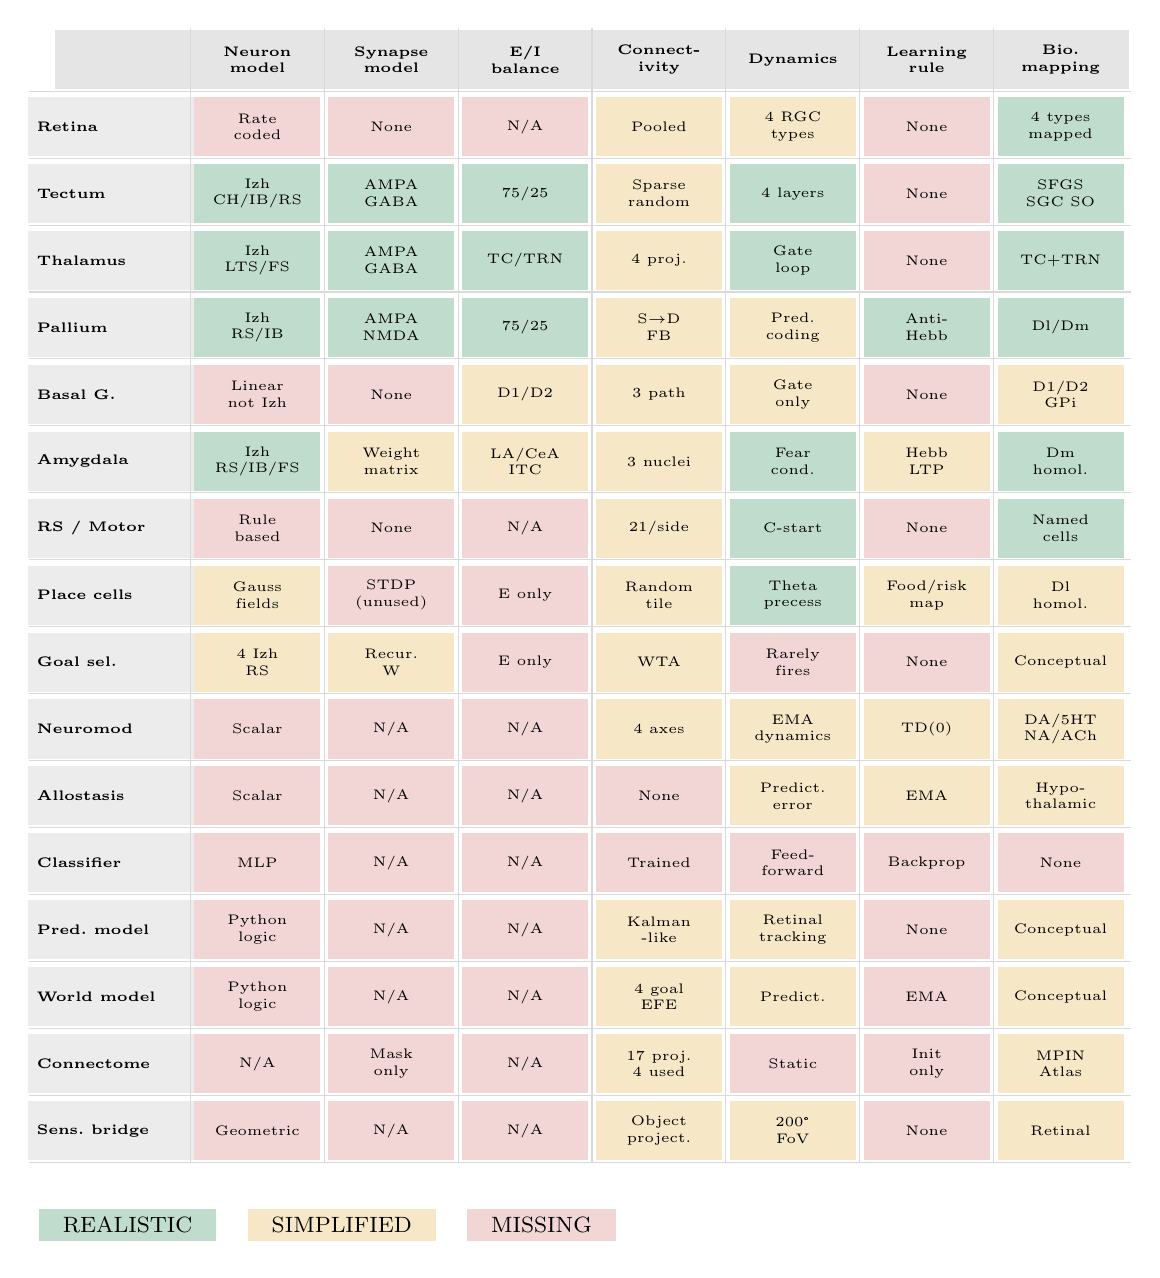
\begin{tikzpicture}[
    cell/.style={minimum width=1.6cm, minimum height=0.75cm, font=\tiny, align=center},
    rcell/.style={cell, fill=realistic!30},
    scell/.style={cell, fill=simplified!25},
    mcell/.style={cell, fill=missing!25},
    hdr/.style={cell, font=\tiny\bfseries, fill=gray!20, text width=1.5cm},
    rhdr/.style={cell, font=\tiny\bfseries, fill=gray!15, text width=2.2cm, align=left},
]

% Column headers
\node[hdr] at (0, 0) {};
\node[hdr] at (1.7, 0) {Neuron\\model};
\node[hdr] at (3.4, 0) {Synapse\\model};
\node[hdr] at (5.1, 0) {E/I\\balance};
\node[hdr] at (6.8, 0) {Connect-\\ivity};
\node[hdr] at (8.5, 0) {Dynamics};
\node[hdr] at (10.2, 0) {Learning\\rule};
\node[hdr] at (11.9, 0) {Bio.\\mapping};

% Row 1: Retina
\node[rhdr] at (0, -0.85) {Retina};
\node[mcell] at (1.7, -0.85) {Rate\\coded};
\node[mcell] at (3.4, -0.85) {None};
\node[mcell] at (5.1, -0.85) {N/A};
\node[scell] at (6.8, -0.85) {Pooled};
\node[scell] at (8.5, -0.85) {4 RGC\\types};
\node[mcell] at (10.2, -0.85) {None};
\node[rcell] at (11.9, -0.85) {4 types\\mapped};

% Row 2: Tectum
\node[rhdr] at (0, -1.7) {Tectum};
\node[rcell] at (1.7, -1.7) {Izh\\CH/IB/RS};
\node[rcell] at (3.4, -1.7) {AMPA\\GABA};
\node[rcell] at (5.1, -1.7) {75/25};
\node[scell] at (6.8, -1.7) {Sparse\\random};
\node[rcell] at (8.5, -1.7) {4 layers};
\node[mcell] at (10.2, -1.7) {None};
\node[rcell] at (11.9, -1.7) {SFGS\\SGC SO};

% Row 3: Thalamus
\node[rhdr] at (0, -2.55) {Thalamus};
\node[rcell] at (1.7, -2.55) {Izh\\LTS/FS};
\node[rcell] at (3.4, -2.55) {AMPA\\GABA};
\node[rcell] at (5.1, -2.55) {TC/TRN};
\node[scell] at (6.8, -2.55) {4 proj.};
\node[rcell] at (8.5, -2.55) {Gate\\loop};
\node[mcell] at (10.2, -2.55) {None};
\node[rcell] at (11.9, -2.55) {TC+TRN};

% Row 4: Pallium
\node[rhdr] at (0, -3.4) {Pallium};
\node[rcell] at (1.7, -3.4) {Izh\\RS/IB};
\node[rcell] at (3.4, -3.4) {AMPA\\NMDA};
\node[rcell] at (5.1, -3.4) {75/25};
\node[scell] at (6.8, -3.4) {S$\to$D\\FB};
\node[scell] at (8.5, -3.4) {Pred.\\coding};
\node[rcell] at (10.2, -3.4) {Anti-\\Hebb};
\node[rcell] at (11.9, -3.4) {Dl/Dm};

% Row 5: BG
\node[rhdr] at (0, -4.25) {Basal G.};
\node[mcell] at (1.7, -4.25) {Linear\\not Izh};
\node[mcell] at (3.4, -4.25) {None};
\node[scell] at (5.1, -4.25) {D1/D2};
\node[scell] at (6.8, -4.25) {3 path};
\node[scell] at (8.5, -4.25) {Gate\\only};
\node[mcell] at (10.2, -4.25) {None};
\node[scell] at (11.9, -4.25) {D1/D2\\GPi};

% Row 6: Amygdala
\node[rhdr] at (0, -5.1) {Amygdala};
\node[rcell] at (1.7, -5.1) {Izh\\RS/IB/FS};
\node[scell] at (3.4, -5.1) {Weight\\matrix};
\node[scell] at (5.1, -5.1) {LA/CeA\\ITC};
\node[scell] at (6.8, -5.1) {3 nuclei};
\node[rcell] at (8.5, -5.1) {Fear\\cond.};
\node[scell] at (10.2, -5.1) {Hebb\\LTP};
\node[rcell] at (11.9, -5.1) {Dm\\homol.};

% Row 7: RS/Motor
\node[rhdr] at (0, -5.95) {RS / Motor};
\node[mcell] at (1.7, -5.95) {Rule\\based};
\node[mcell] at (3.4, -5.95) {None};
\node[mcell] at (5.1, -5.95) {N/A};
\node[scell] at (6.8, -5.95) {21/side};
\node[rcell] at (8.5, -5.95) {C-start};
\node[mcell] at (10.2, -5.95) {None};
\node[rcell] at (11.9, -5.95) {Named\\cells};

% Row 8: Place cells
\node[rhdr] at (0, -6.8) {Place cells};
\node[scell] at (1.7, -6.8) {Gauss\\fields};
\node[mcell] at (3.4, -6.8) {STDP\\(unused)};
\node[mcell] at (5.1, -6.8) {E only};
\node[scell] at (6.8, -6.8) {Random\\tile};
\node[rcell] at (8.5, -6.8) {Theta\\precess};
\node[scell] at (10.2, -6.8) {Food/risk\\map};
\node[scell] at (11.9, -6.8) {Dl\\homol.};

% Row 9: Goal selector
\node[rhdr] at (0, -7.65) {Goal sel.};
\node[scell] at (1.7, -7.65) {4 Izh\\RS};
\node[scell] at (3.4, -7.65) {Recur.\\W};
\node[mcell] at (5.1, -7.65) {E only};
\node[scell] at (6.8, -7.65) {WTA};
\node[mcell] at (8.5, -7.65) {Rarely\\fires};
\node[mcell] at (10.2, -7.65) {None};
\node[scell] at (11.9, -7.65) {Conceptual};

% Row 10: Neuromod
\node[rhdr] at (0, -8.5) {Neuromod};
\node[mcell] at (1.7, -8.5) {Scalar};
\node[mcell] at (3.4, -8.5) {N/A};
\node[mcell] at (5.1, -8.5) {N/A};
\node[scell] at (6.8, -8.5) {4 axes};
\node[scell] at (8.5, -8.5) {EMA\\dynamics};
\node[scell] at (10.2, -8.5) {TD(0)};
\node[scell] at (11.9, -8.5) {DA/5HT\\NA/ACh};

% Row 11: Allostasis
\node[rhdr] at (0, -9.35) {Allostasis};
\node[mcell] at (1.7, -9.35) {Scalar};
\node[mcell] at (3.4, -9.35) {N/A};
\node[mcell] at (5.1, -9.35) {N/A};
\node[mcell] at (6.8, -9.35) {None};
\node[scell] at (8.5, -9.35) {Predict.\\error};
\node[scell] at (10.2, -9.35) {EMA};
\node[scell] at (11.9, -9.35) {Hypo-\\thalamic};

% Row 12: Classifier
\node[rhdr] at (0, -10.2) {Classifier};
\node[mcell] at (1.7, -10.2) {MLP};
\node[mcell] at (3.4, -10.2) {N/A};
\node[mcell] at (5.1, -10.2) {N/A};
\node[mcell] at (6.8, -10.2) {Trained};
\node[mcell] at (8.5, -10.2) {Feed-\\forward};
\node[mcell] at (10.2, -10.2) {Backprop};
\node[mcell] at (11.9, -10.2) {None};

% Row 13: Pred model
\node[rhdr] at (0, -11.05) {Pred.\ model};
\node[mcell] at (1.7, -11.05) {Python\\logic};
\node[mcell] at (3.4, -11.05) {N/A};
\node[mcell] at (5.1, -11.05) {N/A};
\node[scell] at (6.8, -11.05) {Kalman\\-like};
\node[scell] at (8.5, -11.05) {Retinal\\tracking};
\node[mcell] at (10.2, -11.05) {None};
\node[scell] at (11.9, -11.05) {Conceptual};

% Row 14: World model
\node[rhdr] at (0, -11.9) {World model};
\node[mcell] at (1.7, -11.9) {Python\\logic};
\node[mcell] at (3.4, -11.9) {N/A};
\node[mcell] at (5.1, -11.9) {N/A};
\node[scell] at (6.8, -11.9) {4 goal\\EFE};
\node[scell] at (8.5, -11.9) {Predict.};
\node[mcell] at (10.2, -11.9) {EMA};
\node[scell] at (11.9, -11.9) {Conceptual};

% Row 15: Connectome
\node[rhdr] at (0, -12.75) {Connectome};
\node[mcell] at (1.7, -12.75) {N/A};
\node[mcell] at (3.4, -12.75) {Mask\\only};
\node[mcell] at (5.1, -12.75) {N/A};
\node[scell] at (6.8, -12.75) {17 proj.\\4 used};
\node[mcell] at (8.5, -12.75) {Static};
\node[mcell] at (10.2, -12.75) {Init\\only};
\node[scell] at (11.9, -12.75) {MPIN\\Atlas};

% Row 16: Sensory bridge
\node[rhdr] at (0, -13.6) {Sens.\ bridge};
\node[mcell] at (1.7, -13.6) {Geometric};
\node[mcell] at (3.4, -13.6) {N/A};
\node[mcell] at (5.1, -13.6) {N/A};
\node[scell] at (6.8, -13.6) {Object\\project.};
\node[scell] at (8.5, -13.6) {200\textdegree\\FoV};
\node[mcell] at (10.2, -13.6) {None};
\node[scell] at (11.9, -13.6) {Retinal};

% Legend
\node[font=\footnotesize, anchor=west] at (-1.2, -14.8) {
\colorbox{realistic!30}{\textcolor{black}{~~REALISTIC~~}}
\quad
\colorbox{simplified!25}{\textcolor{black}{~~SIMPLIFIED~~}}
\quad
\colorbox{missing!25}{\textcolor{black}{~~MISSING~~}}
};

% Grid lines
\foreach \y in {-0.4, -1.25, -2.1, -2.95, -3.8, -4.65, -5.5, -6.35, -7.2, -8.05, -8.9, -9.75, -10.6, -11.45, -12.3, -13.15, -14.0} {
  \draw[gray!30] (-1.2, \y) -- (12.8, \y);
}
\foreach \x in {0.85, 2.55, 4.25, 5.95, 7.65, 9.35, 11.05} {
  \draw[gray!30] (\x, 0.4) -- (\x, -14.0);
}
\end{tikzpicture}
}
\caption{Biological plausibility matrix.  Green = realistic implementation matching
known biology.  Yellow = simplified but conceptually grounded.  Red = missing or
non-biological implementation.}
\label{fig:matrix}
\end{figure}

\noindent\textbf{Counting cells:} Of the 112 cells in the matrix (16 components $\times$ 7 criteria),
approximately 22 (20\%) are \textcolor{realistic}{REALISTIC},
38 (34\%) are \textcolor{simplified}{SIMPLIFIED}, and
52 (46\%) are \textcolor{missing}{MISSING}.
The strongest biological fidelity is in the tectum and thalamus modules;
the weakest is in non-neural components (classifier, world model, sensory bridge).

%% ========================================================================
\section{Conclusions and Recommendations}
\label{sec:conclusions}

\subsection{What Is Genuinely Biologically Plausible (Ranked)}

\begin{enumerate}[leftmargin=*]
\item \textbf{E/I layer architecture with conductance-based synapses.}
  The \texttt{EILayer} abstraction with 75/25 E/I ratio, AMPA/NMDA/GABA\textsubscript{A}
  conductances, and Mg$^{2+}$ block represents a solid biophysical foundation that
  is consistent with vertebrate cortical microcircuits.

\item \textbf{Tectum layered organization.}
  Four functional layers (SFGS-b, SFGS-d, SGC, SO) with distinct cell types
  (CH superficial, IB deep, RS stratum opticum) match the known laminar
  organization of the zebrafish optic tectum.

\item \textbf{Thalamic relay with TRN gating.}
  The TC/TRN circuit with NA-modulated wake/sleep bias correctly implements
  the thalamic relay function.

\item \textbf{Mauthner cell C-start escape.}
  The 4-step motor sequence with looming trigger, refractory period, and BG
  gate bypass faithfully reproduces the hallmark zebrafish escape behavior.

\item \textbf{Two-compartment predictive coding in pallium.}
  Apical-somatic mismatch with anti-Hebbian feedback learning is consistent
  with modern theories of cortical predictive processing.

\item \textbf{Allostatic interoceptive regulation.}
  Three-axis interoception with predictive errors and starvation--safety
  trade-off demonstrates the most ecologically impactful module.

\item \textbf{4-RGC-type retinal encoding.}
  ON/OFF/Looming/Direction-selective types capture the functional diversity
  of retinal output.
\end{enumerate}

\subsection{Biggest Gaps}

\begin{enumerate}[leftmargin=*]
\item \textbf{Analytic EFE dominates spiking dynamics.}
  The brain's spiking substrate is largely decorative: goal selection,
  motor commands, and sensory processing all rely on hand-coded formulas
  that bypass the neural network.  The spiking WTA goal selector fires
  $<$5\% of the time and behavior falls back to \texttt{argmax(EFE)}.

\item \textbf{Missing brain regions.}
  Habenula (reward aversion, learned helplessness), cerebellum
  (motor timing, sensory prediction), and hypothalamus (homeostatic control)
  are absent despite their well-characterized roles in zebrafish behavior.

\item \textbf{Point neurons without dendrites.}
  The Izhikevich model captures somatic dynamics but misses dendritic
  computation, which is critical for coincidence detection, nonlinear
  integration, and calcium-dependent plasticity.

\item \textbf{50$\times$ scale reduction.}
  7,369 neurons cannot support the population dynamics (traveling waves,
  attractor manifolds, oscillatory synchronization) that emerge in
  the real 100K-neuron brain.

\item \textbf{Connectome constraints are cosmetic.}
  Only 4 of 17 defined projections are actually used, and none employ
  topographic mapping, distance-dependent connectivity, or hemispheric
  laterality from the loaded atlas data.
\end{enumerate}

\subsection{Priority Fixes for Biological Realism}

\begin{enumerate}[leftmargin=*]
\item \textbf{P1: Make spiking dynamics drive behavior.}
  Replace analytic EFE with population-coded belief updates through the
  thalamo-pallial loop.  Train the spiking WTA to self-organize goal
  selection through STDP, eliminating the \texttt{argmax} fallback.

\item \textbf{P2: Implement cerebellum.}
  Add a granule cell$\to$Purkinje cell$\to$deep cerebellar nucleus circuit
  for motor timing and sensory prediction error.  This would enable
  forward model-based motor learning.

\item \textbf{P3: Implement habenula.}
  Add lateral and medial habenula with habenula$\to$raphe 5-HT modulation
  for learned behavioral suppression and aversion.

\item \textbf{P4: Spiking BG.}
  Replace \texttt{nn.Linear} BG with spiking MSN populations using the
  already-defined MSN Izhikevich type.

\item \textbf{P5: Topographic connectome.}
  Use atlas centroid coordinates to create retinotopic retina$\to$tectum
  mapping and distance-dependent connectivity for all projections.

\item \textbf{P6: Spiking retina.}
  Replace rate-coded RGCs with spiking populations to enable temporal
  coding and spike-timing-dependent computations in tectum.

\item \textbf{P7: Scale to 50K neurons.}
  GPU-optimized sparse matrix operations could support 50K Izhikevich
  neurons at real-time speeds, bringing the model within an order of
  magnitude of the biological neuron count.
\end{enumerate}

\subsection{Comparison to Other Zebrafish Models}

\begin{table}[H]
\centering
\caption{Comparison with published zebrafish computational models.}
\label{tab:comparison}
\begin{tabular}{@{}lcccc@{}}
\toprule
\textbf{Feature} & \textbf{This work} & \textbf{Dragomir} & \textbf{Randlett} & \textbf{Dunn} \\
 & \textbf{(v2)} & \textbf{et al.\ 2020} & \textbf{et al.\ 2015} & \textbf{et al.\ 2016} \\
\midrule
Neuron model     & Izhikevich    & Rate/LIF        & Correlation  & GLM \\
Spiking          & Yes           & Partial         & No           & No \\
Neuron count     & 7,369         & $\sim$100       & Whole brain  & $\sim$80K \\
Connectome       & MPIN partial  & Hand-coded      & Activity map & Activity map \\
Behavior         & Closed-loop   & Open-loop       & Open-loop    & Closed-loop \\
Active inference & Analytic EFE  & No              & No           & No \\
Motor control    & Mauthner+RS   & No              & No           & Tail kinematics \\
Neuromodulation  & 4-axis scalar & DA only         & No           & No \\
Senses           & Vision+LL     & Vision          & Whole brain  & Vision \\
\bottomrule
\end{tabular}
\end{table}

\noindent The v2 model is unique in combining spiking neural dynamics with
closed-loop behavior, active inference, and named reticulospinal neurons.
However, it sacrifices neural realism for behavioral breadth: models like
Dunn et al.\ (2016) achieve much higher neuron counts through whole-brain
calcium imaging constraints, while Randlett et al.\ (2015) provide atlas-registered
activity maps that could directly inform future versions.

\subsection{Final Assessment}

The Virtual Zebrafish Brain v2 represents a principled attempt to bridge
computational neuroscience theory (predictive coding, active inference,
three-factor STDP) with systems neuroscience data (MapZebrain atlas,
identified reticulospinal neurons, RGC types).  Its 77/100 decision quality
score demonstrates that the behavioral architecture is competent.
However, the honest assessment is that the spiking neural network substrate
is largely bypassed by analytic formulas for the critical computations
(goal selection, motor planning, sensory interpretation).
The path to genuine biological plausibility requires making the spiking dynamics
\emph{do the work}---replacing hand-coded formulas with emergent computation
in neural populations constrained by connectome data.

\bigskip
\noindent\textbf{Overall biological plausibility score:}
On a scale from pure engineering (0) to biophysically faithful (10),
we rate the v2 model at approximately \textbf{4/10}: the architectural
skeleton maps onto real zebrafish neuroanatomy, but the computational
substance remains largely algorithmic rather than neural.

%% ========================================================================
\subsection*{References}

\begin{small}
\noindent
Barrett, L.F.\ \& Simmons, W.K.\ (2015). Interoceptive predictions in the brain.
\textit{Nature Reviews Neuroscience}, 16(7), 419--429.

\noindent
Bianco, I.H.\ \& Engert, F.\ (2015). Visuomotor transformations underlying hunting behavior in zebrafish.
\textit{Current Biology}, 25(7), 831--846.

\noindent
Bianco, I.H., Kampff, A.R., \& Engert, F.\ (2011). Prey capture behavior evoked by simple visual stimuli in larval zebrafish.
\textit{Frontiers in Systems Neuroscience}, 5, 101.

\noindent
Crick, F.\ (1984). Function of the thalamic reticular complex: the searchlight hypothesis.
\textit{PNAS}, 81(14), 4586--4590.

\noindent
Dragomir, E.I., \v{S}v\'ara, V., \& Bhatt, D.H.\ (2020). Evidence accumulation during a sensorimotor decision task revealed by whole-brain imaging.
\textit{Nature Neuroscience}, 23(1), 85--93.

\noindent
Dunn, T.W.\ et al.\ (2016). Brain-wide mapping of neural activity controlling zebrafish exploratory locomotion.
\textit{eLife}, 5, e12741.

\noindent
F\"orster, D.\ et al.\ (2017). Genetic targeting and anatomical registration of neuronal populations in the zebrafish brain.
\textit{Nature Methods}, 14(11), 1025--1030.

\noindent
Friston, K.\ (2010). The free-energy principle: a unified brain theory?
\textit{Nature Reviews Neuroscience}, 11(2), 127--138.

\noindent
Halassa, M.M.\ \& Kastner, S.\ (2017). Thalamic functions in distributed cognitive control.
\textit{Nature Neuroscience}, 20(12), 1669--1679.

\noindent
Izhikevich, E.M.\ (2003). Simple model of spiking neurons.
\textit{IEEE Transactions on Neural Networks}, 14(6), 1569--1572.

\noindent
Kimmel, C.B., Powell, S.L., \& Metcalfe, W.K.\ (1982). Brain neurons which project to the spinal cord in young larvae of the zebrafish.
\textit{Journal of Comparative Neurology}, 205(2), 112--127.

\noindent
Kinkhabwala, A.\ et al.\ (2011). A structural and functional ground plan for neurons in the hindbrain of zebrafish.
\textit{PNAS}, 108(3), 1164--1169.

\noindent
Kunst, M.\ et al.\ (2019). A cellular-resolution atlas of the larval zebrafish brain.
\textit{Neuron}, 103(1), 21--38.

\noindent
Mu, Y.\ et al.\ (2019). Glia accumulate evidence that actions are futile and suppress unsuccessful behavior.
\textit{Cell}, 178(1), 27--43.

\noindent
Randlett, O.\ et al.\ (2015). Whole-brain activity mapping onto a zebrafish brain atlas.
\textit{Nature Methods}, 12(11), 1039--1046.

\noindent
Reynolds, J.H.\ \& Heeger, D.J.\ (2009). The normalization model of attention.
\textit{Neuron}, 61(2), 168--185.

\noindent
Sacramento, J.\ et al.\ (2018). Dendritic cortical microcircuits approximate the backpropagation algorithm.
\textit{NeurIPS}, 31.

\noindent
Schultz, W., Dayan, P., \& Montague, P.R.\ (1997). A neural substrate of prediction and reward.
\textit{Science}, 275(5306), 1593--1599.

\noindent
Seth, A.K.\ (2013). Interoceptive inference, emotion, and the embodied self.
\textit{Trends in Cognitive Sciences}, 17(11), 565--573.

\noindent
Sterling, P.\ (2012). Allostasis: a model of predictive regulation.
\textit{Physiology \& Behavior}, 106(1), 5--15.
\end{small}

\end{document}
